%%%%%%%%%%%%%%%%%%%%%%%%%%%%%%%%%%%%%%%%%
% Programming/Coding Assignment
% LaTeX Template
%
% This template has been downloaded from:
% http://www.latextemplates.com
%
% Original author:
% Ted Pavlic (http://www.tedpavlic.com)
%
% Note:
% The \lipsum[#] commands throughout this template generate dummy text
% to fill the template out. These commands should all be removed when 
% writing assignment content.
%
% This template uses a Perl script as an example snippet of code, most other
% languages are also usable. Configure them in the "CODE INCLUSION 
% CONFIGURATION" section.
%
%%%%%%%%%%%%%%%%%%%%%%%%%%%%%%%%%%%%%%%%%

%----------------------------------------------------------------------------------------
%	PACKAGES AND OTHER DOCUMENT CONFIGURATIONS
%----------------------------------------------------------------------------------------

\documentclass[a4paper]{article}

\usepackage{fancyhdr} % Required for custom headers
\usepackage{lastpage} % Required to determine the last page for the footer
\usepackage{extramarks} % Required for headers and footers
\usepackage[usenames,dvipsnames]{color} % Required for custom colors
\usepackage{graphicx} % Required to insert images
\usepackage{listings} % Required for insertion of code
\usepackage{courier} % Required for the courier font
\usepackage{lipsum} % Used for inserting dummy 'Lorem ipsum' text into the template
\usepackage{multirow}
\usepackage{tabu}
\usepackage{float}
\usepackage{pbox}

% Margins
\topmargin=-0.45in
\evensidemargin=0in
\oddsidemargin=0in
\textwidth=6.5in
\textheight=9.5in
\headsep=0.25in

\linespread{1.1} % Line spacing

% Set up the header and footer
\pagestyle{fancy}
\lhead{\hmwkAuthorName} % Top left header
\chead{\hmwkShortTitle} % Top center head
\rhead{\firstxmark} % Top right header
\lfoot{\lastxmark} % Bottom left footer
\cfoot{} % Bottom center footer
\rfoot{Page\ \thepage\ of\ \protect\pageref{LastPage}} % Bottom right footer
\renewcommand\headrulewidth{0.4pt} % Size of the header rule
\renewcommand\footrulewidth{0.4pt} % Size of the footer rule

\setlength\parindent{0pt} % Removes all indentation from paragraphs

%----------------------------------------------------------------------------------------
%	CODE INCLUSION CONFIGURATION
%----------------------------------------------------------------------------------------

\definecolor{MyDarkGreen}{rgb}{0.0,0.4,0.0} % This is the color used for comments
\lstloadlanguages{Matlab} % Load Perl syntax for listings, for a list of other languages supported see: ftp://ftp.tex.ac.uk/tex-archive/macros/latex/contrib/listings/listings.pdf
\lstset{language=Matlab, % Use Perl in this example
        frame=single, % Single frame around code
        basicstyle=\small\ttfamily, % Use small true type font
        keywordstyle=[1]\color{Blue}\bf, % Perl functions bold and blue
        keywordstyle=[2]\color{Purple}, % Perl function arguments purple
        keywordstyle=[3]\color{Blue}\underbar, % Custom functions underlined and blue
        identifierstyle=, % Nothing special about identifiers                                         
        commentstyle=\usefont{T1}{pcr}{m}{sl}\color{MyDarkGreen}\small, % Comments small dark green courier font
        stringstyle=\color{Purple}, % Strings are purple
        showstringspaces=false, % Don't put marks in string spaces
        tabsize=5, % 5 spaces per tab
        %
        % Put standard Perl functions not included in the default language here
        morekeywords={rand},
        %
        % Put Perl function parameters here
        morekeywords=[2]{on, off, interp},
        %
        % Put user defined functions here
        morekeywords=[3]{test},
       	%
        morecomment=[l][\color{Blue}]{...}, % Line continuation (...) like blue comment
        numbers=left, % Line numbers on left
        firstnumber=1, % Line numbers start with line 1
        numberstyle=\tiny\color{Blue}, % Line numbers are blue and small
        stepnumber=5 % Line numbers go in steps of 5
}

% Creates a new command to include a perl script, the first parameter is the filename of the script (without .pl), the second parameter is the caption
\newcommand{\matlabscript}[2]{
\begin{itemize}
\item[]\lstinputlisting[caption=#2,label=#1]{#1.m}
\end{itemize}
}

%----------------------------------------------------------------------------------------
%	DOCUMENT STRUCTURE COMMANDS
%	Skip this unless you know what you're doing
%----------------------------------------------------------------------------------------

% Header and footer for when a page split occurs within a problem environment
\newcommand{\enterProblemHeader}[1]{
\nobreak\extramarks{#1}{#1 continued on next page\ldots}\nobreak
\nobreak\extramarks{#1 (continued)}{#1 continued on next page\ldots}\nobreak
}

% Header and footer for when a page split occurs between problem environments
\newcommand{\exitProblemHeader}[1]{
\nobreak\extramarks{#1 (continued)}{#1 continued on next page\ldots}\nobreak
\nobreak\extramarks{#1}{}\nobreak
}

\setcounter{secnumdepth}{0} % Removes default section numbers
\newcounter{homeworkProblemCounter} % Creates a counter to keep track of the number of problems

\newcommand{\homeworkProblemName}{}
\newenvironment{homeworkProblem}[1][Problem \arabic{homeworkProblemCounter}]{ % Makes a new environment called homeworkProblem which takes 1 argument (custom name) but the default is "Problem #"
\stepcounter{homeworkProblemCounter} % Increase counter for number of problems
\renewcommand{\homeworkProblemName}{#1} % Assign \homeworkProblemName the name of the problem
\section{\homeworkProblemName} % Make a section in the document with the custom problem count
\enterProblemHeader{\homeworkProblemName} % Header and footer within the environment
}{
\exitProblemHeader{\homeworkProblemName} % Header and footer after the environment
}

\newcommand{\problemAnswer}[1]{ % Defines the problem answer command with the content as the only argument
\noindent\framebox[\columnwidth][c]{\begin{minipage}{0.98\columnwidth}#1\end{minipage}} % Makes the box around the problem answer and puts the content inside
}

\newcommand{\homeworkSectionName}{}
\newenvironment{homeworkSection}[1]{ % New environment for sections within homework problems, takes 1 argument - the name of the section
\renewcommand{\homeworkSectionName}{#1} % Assign \homeworkSectionName to the name of the section from the environment argument
\subsection{\homeworkSectionName} % Make a subsection with the custom name of the subsection
\enterProblemHeader{\homeworkProblemName\ [\homeworkSectionName]} % Header and footer within the environment
}{
\enterProblemHeader{\homeworkProblemName} % Header and footer after the environment
}

%----------------------------------------------------------------------------------------
%	NAME AND CLASS SECTION
%----------------------------------------------------------------------------------------

\newcommand{\hmwkTitle}{CO395 Machine Learning\\CBC \#1\\Decision Trees} % Assignment title
\newcommand{\hmwkShortTitle}{CBC \#1 - Decision Trees}
\newcommand{\hmwkDueDate}{Monday,\ November\ 4,\ 2013} % Due date
\newcommand{\hmwkAuthorName}{Group 1} % Your name

%----------------------------------------------------------------------------------------
%	TITLE PAGE
%----------------------------------------------------------------------------------------

\title{
\vspace{2in}
\textmd{\textbf{\hmwkTitle}}\\
%\normalsize\vspace{0.1in}\small{Due\ on\ \hmwkDueDate}\\
%\vspace{0.1in}\large{\textit{\hmwkClassInstructor\ \hmwkClassTime}}
\vspace{3in}
\textbf{Group 1}\\
Yong Wen Chua, \texttt{ywc110}\\
Thomas Morrison, \texttt{tm1810}\\
Marcin Baginski, \texttt{mgb10}\\
Marcin Kadziela, \texttt{mk4910}
}

%\author{\textbf{\hmwkAuthorName}}

\date{} % Insert date here if you want it to appear below your name

%----------------------------------------------------------------------------------------

\begin{document}

\maketitle

%----------------------------------------------------------------------------------------
%	TABLE OF CONTENTS
%----------------------------------------------------------------------------------------

%\setcounter{tocdepth}{1} % Uncomment this line if you don't want subsections listed in the ToC

\newpage
\tableofcontents
\newpage

%----------------------------------------------------------------------------------------
%	EXAMPLES
%----------------------------------------------------------------------------------------

% Example how to paste code into the report:
%
% Listing \ref{LIFDemo} shows a Matlab script.
% \matlabscript{LIFDemo}{Sample Perl Script With Highlighting}

% Example how to paste a figure into the report:
% \begin{figure}
% \center
% 
\includegraphics[width=0.75\columnwidth]{example_figure} % Example image
% \caption{sometext}
% \end{figure}

% Ready code for the confusion matrix:
%
%\begin{table}
%\center
%\begin{tabu}{cc|c|c|c|c|c|c|}
%\cline{3-8}
%& & \multicolumn{6}{ c| }{Predicted class} \\ \cline{3-8}
%& & 1 & 2 & 3 & 4 & 5 & 6 \\ \cline{1-2} \tabucline[1.5pt]{3-8}
%\multicolumn{1}{ |c| }{\multirow{6}{*}{Actual class} } &
%\multicolumn{1}{ |c|[1.5pt] }{1} & 0 & 0 & 0 & 0 & 0 & 0     \\ \cline{2-8}
%\multicolumn{1}{ |c| }{}                        &
%\multicolumn{1}{ |c|[1.5pt] }{2} & 0 & 0 & 0 & 0 & 0 & 0     \\ \cline{2-8}
%\multicolumn{1}{ |c|  }{}                        &
%\multicolumn{1}{ |c|[1.5pt] }{3} & 0 & 0 & 0 & 0 & 0 & 0     \\ \cline{2-8}
%\multicolumn{1}{ |c|  }{}                        &
%\multicolumn{1}{ |c|[1.5pt] }{4} & 0 & 0 & 0 & 0 & 0 & 0     \\ \cline{2-8}
%\multicolumn{1}{ |c|  }{}                        &
%\multicolumn{1}{ |c|[1.5pt] }{5} & 0 & 0 & 0 & 0 & 0 & 0     \\ \cline{2-8}
%\multicolumn{1}{ |c|  }{}                        &
%\multicolumn{1}{ |c|[1.5pt] }{6} & 0 & 0 & 0 & 0 & 0 & 0     \\ \cline{1-8}
%\end{tabu}
%\caption{Confusion Matrix}
%\label{confusionMatrix}
%\end{table}

%----------------------------------------------------------------------------------------
%	SECTION 1 - Implementation Details
%----------------------------------------------------------------------------------------

\section{Implementation Details}

\clearpage

%----------------------------------------------------------------------------------------
%	SECTION 2 - Tree Figures
%----------------------------------------------------------------------------------------

\section{Tree Figures}

\subsection{Emotion 1 - Anger}
\begin{figure}[H]
\center
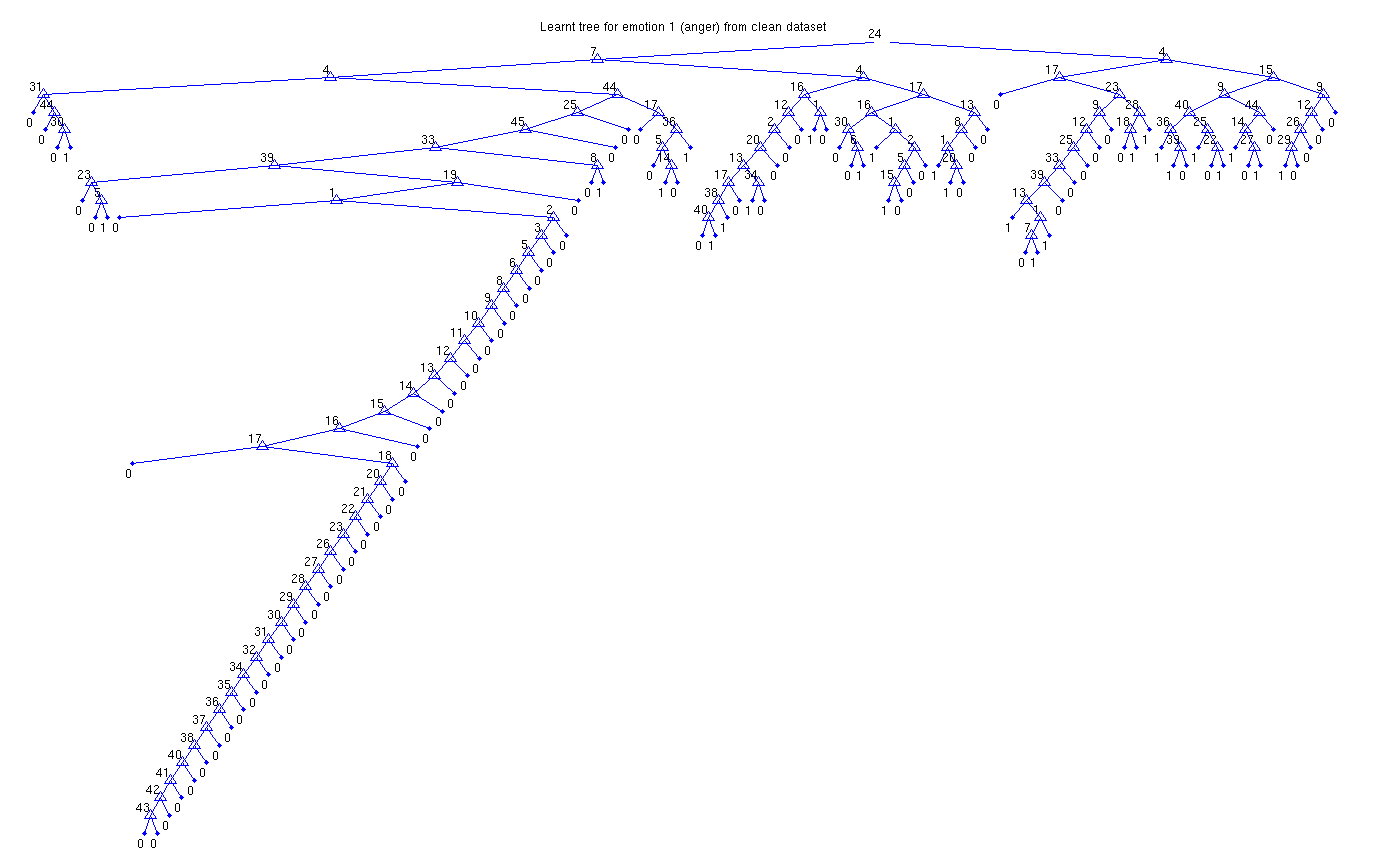
\includegraphics[width=0.9\columnwidth]{AngerTree} % Example image
\caption{Trained decsion tree on the clean dataset for emotion 1 (anger)}
\end{figure}

%\bigskip\bigskip\bigskip\bigskip\bigskip\bigskip
\subsection{Emotion 2 - Disgust}
\begin{figure}[H]
\center
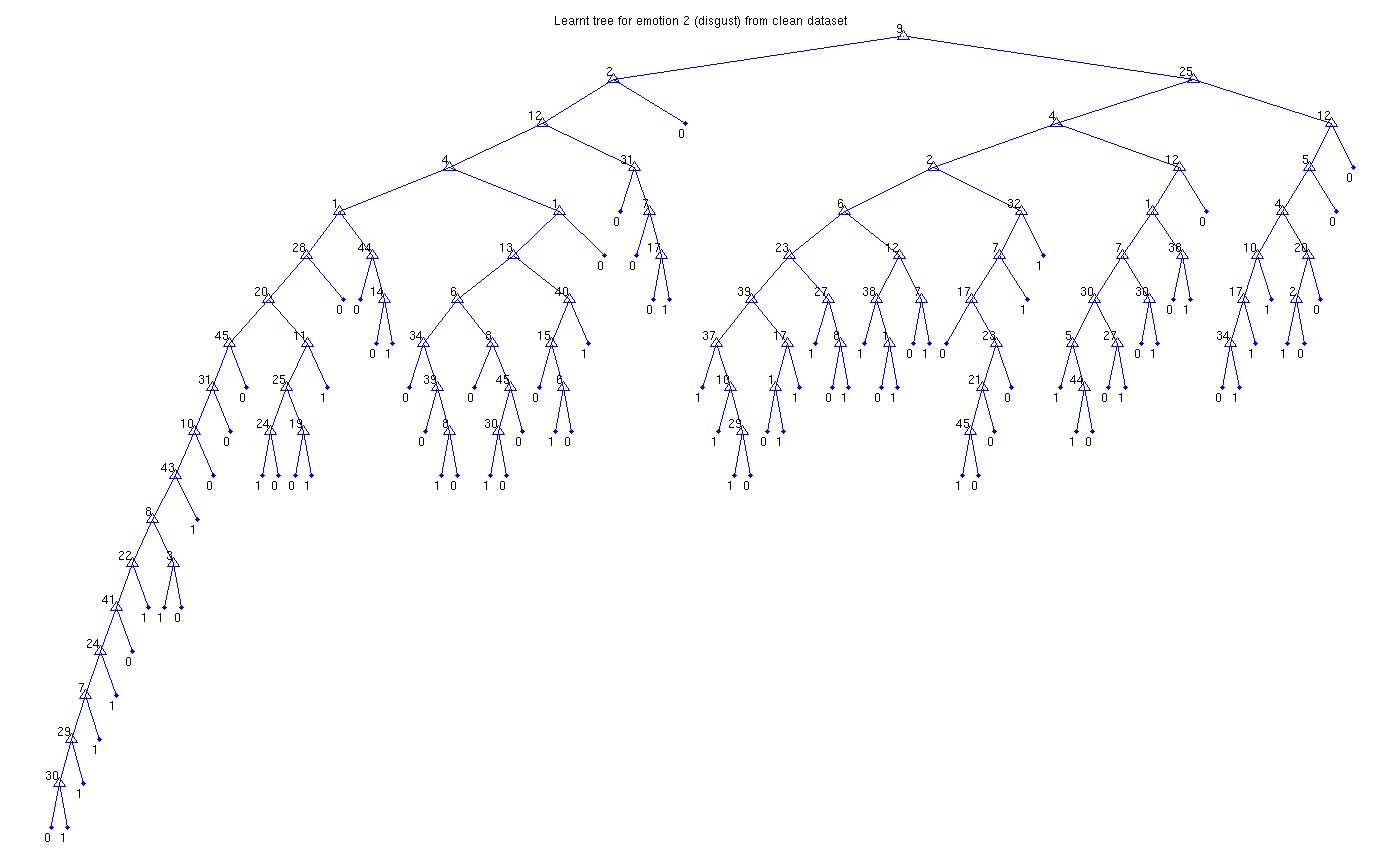
\includegraphics[width=0.9\columnwidth]{DisgustTree} % Example image
\caption{Trained decsion tree on the clean dataset for emotion 2 (disgust)}
\end{figure}

\subsection{Emotion 3 - Fear}
\begin{figure}[H]
\center
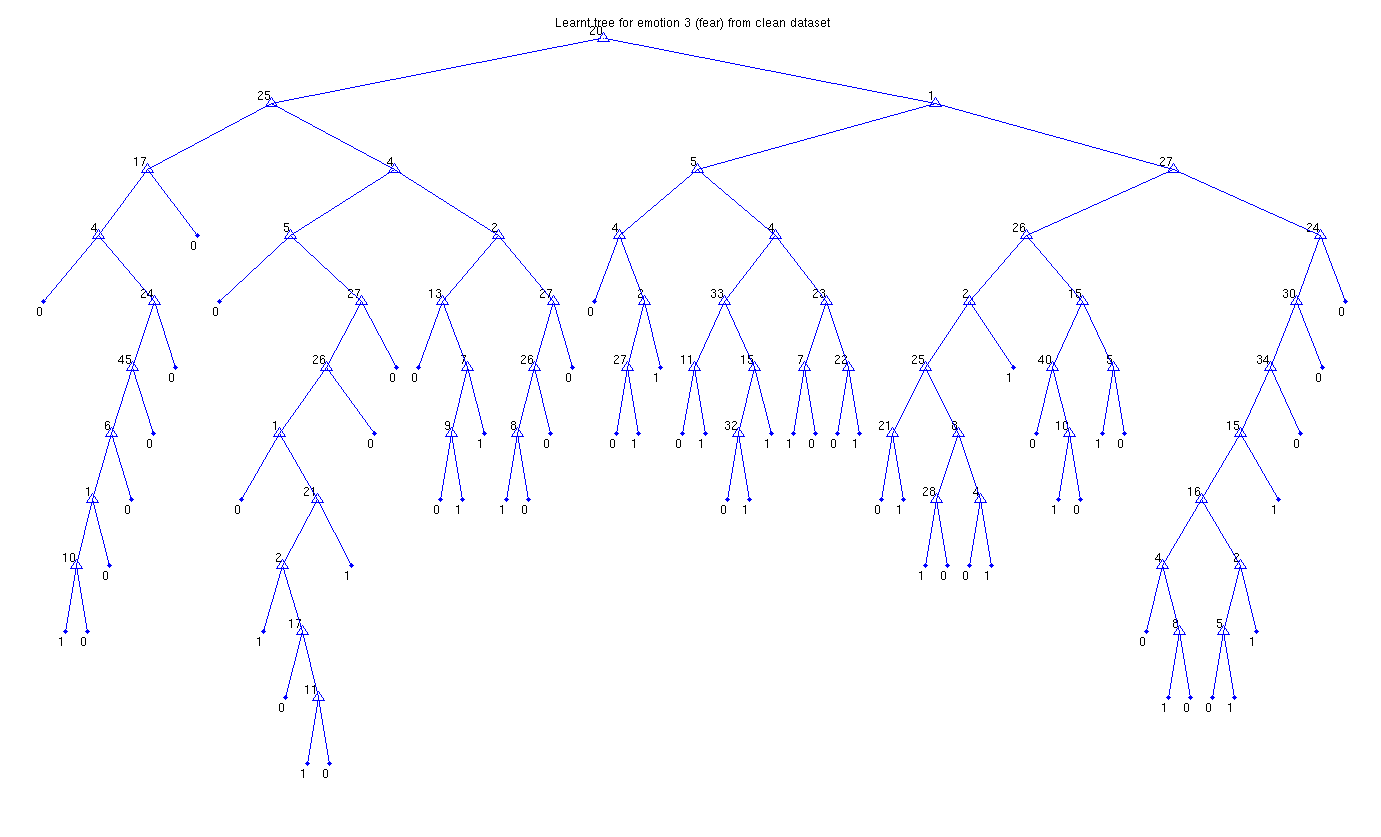
\includegraphics[width=0.9\columnwidth]{FearTree} % Example image
\caption{Trained decsion tree on the clean dataset for emotion 3 (fear)}
\end{figure}

\bigskip\bigskip\bigskip\bigskip\bigskip\bigskip
\subsection{Emotion 4 - Happiness}
\begin{figure}[H]
\center
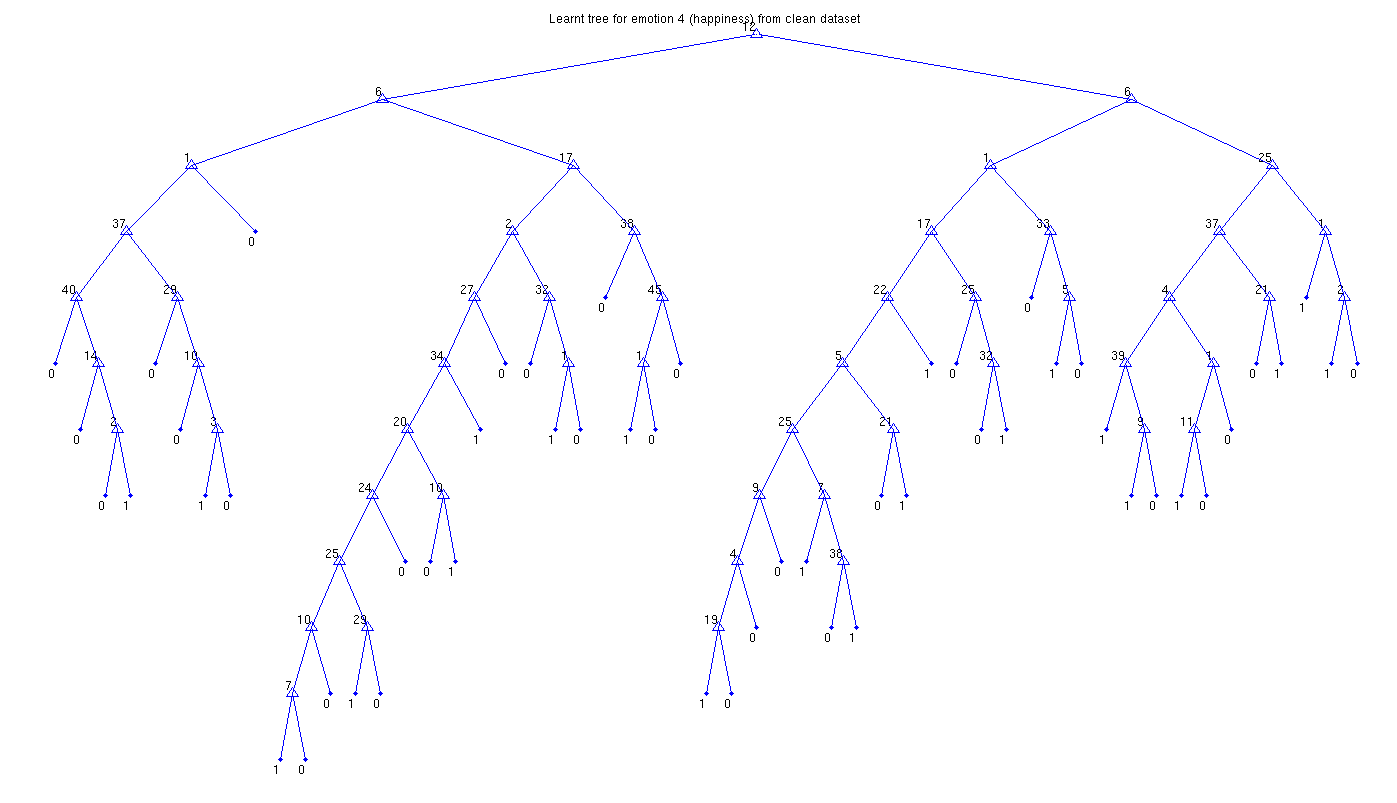
\includegraphics[width=0.9\columnwidth]{HappinessTree} % Example image
\caption{Trained decsion tree on the clean dataset for emotion 4 (happiness)}
\end{figure}

\subsection{Emotion 5 - Sadness}
\begin{figure}[H]
\center
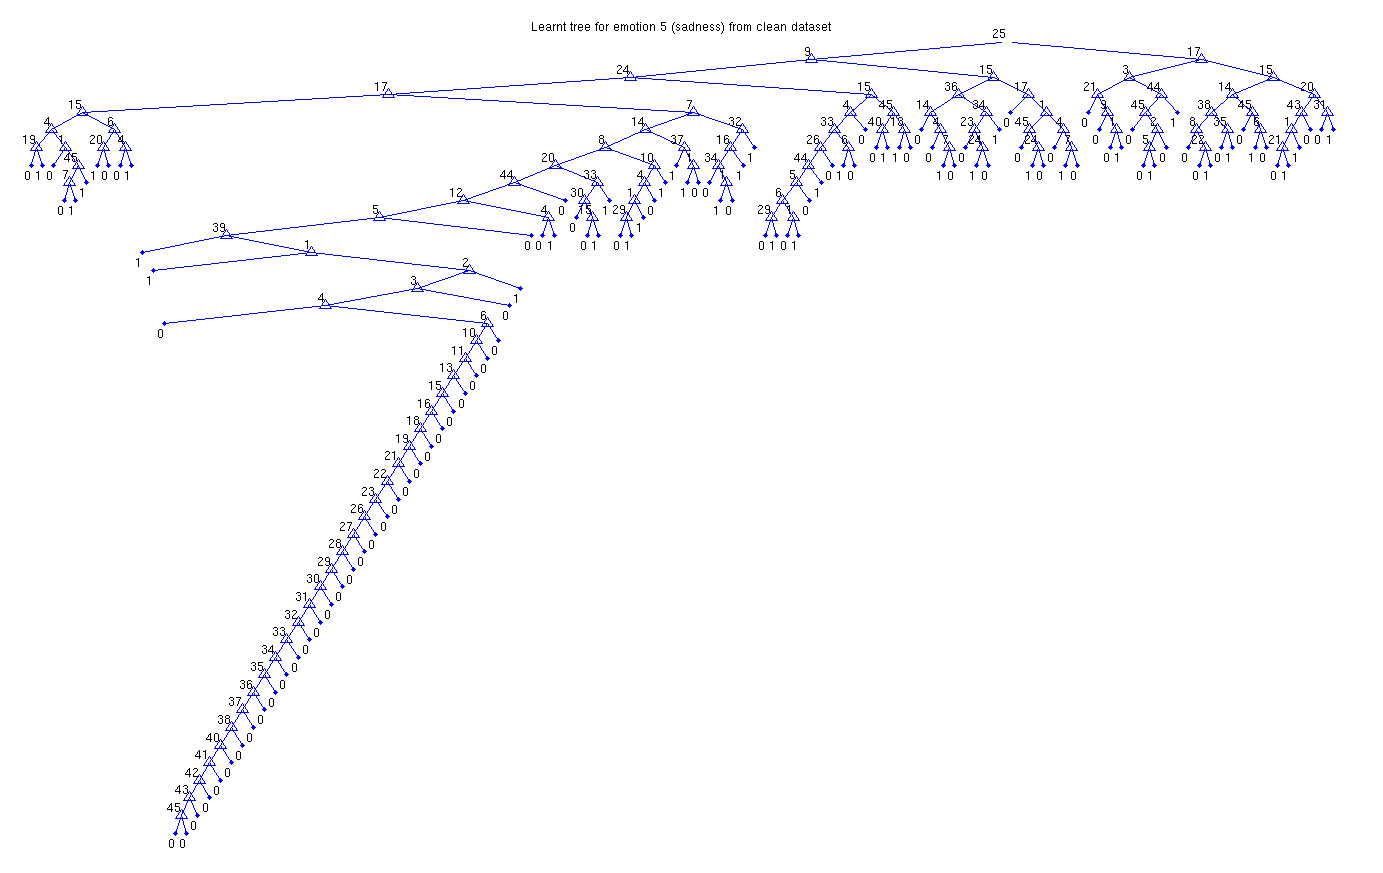
\includegraphics[width=0.9\columnwidth]{SadnessTree} % Example image
\caption{Trained decsion tree on the clean dataset for emotion 5 (sadness)}
\end{figure}

\bigskip\bigskip\bigskip\bigskip\bigskip\bigskip
\subsection{Emotion 6 - Surprise}
\begin{figure}[H]
\center
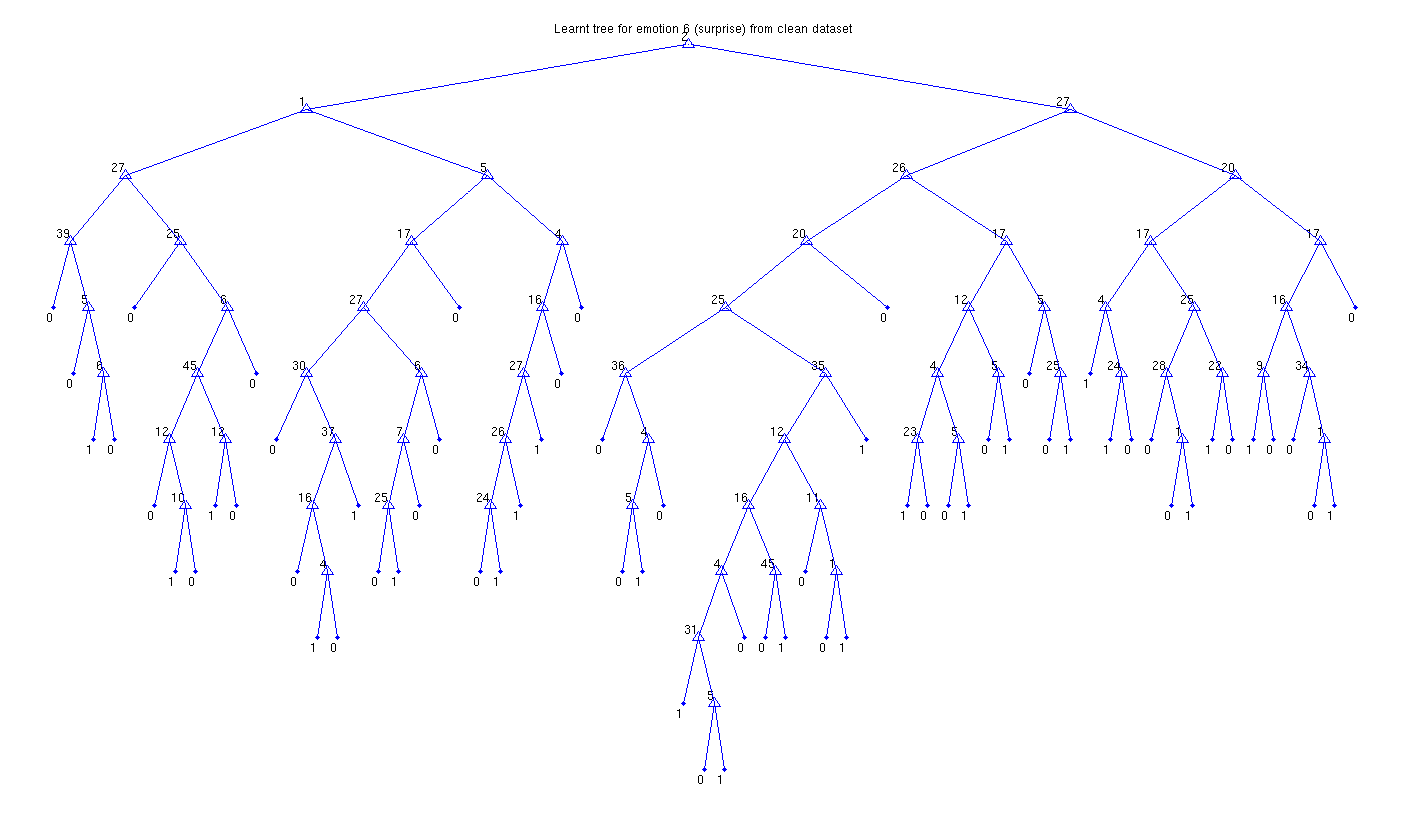
\includegraphics[width=0.9\columnwidth]{SurpriseTree} % Example image
\caption{Trained decsion tree on the clean dataset for emotion 6 (surprise)}
\end{figure}

\clearpage

%----------------------------------------------------------------------------------------
%	SECTION 3 - Evaluation
%----------------------------------------------------------------------------------------

\section{Evaluation}

The results presented below are for a random assignment of conflicted classifications. Evaluation of other strategies is presented in the next section.

\subsection{Clean dataset}
\subsubsection{Confusion matrix}

\begin{table}[H]
\center
\begin{tabu}{cc|c|c|c|c|c|c|}
\cline{3-8}
& & \multicolumn{6}{ c| }{Predicted class} \\ \cline{3-8}
& & 1 & 2 & 3 & 4 & 5 & 6 \\ \cline{1-2} \tabucline[1.5pt]{3-8}
\multicolumn{1}{ |c| }{\multirow{6}{*}{Actual class} } &
\multicolumn{1}{ |c|[1.5pt] }{1} & \textbf{85} & 15 & 4 & 9 & 17 & 2 \\ \cline{2-8}
\multicolumn{1}{ |c| }{}                        &
\multicolumn{1}{ |c|[1.5pt] }{2} & 17 & \textbf{137} & 5 & 12 & 15 & 12 \\ \cline{2-8}
\multicolumn{1}{ |c|  }{}                        &
\multicolumn{1}{ |c|[1.5pt] }{3} & 8 & 7 & \textbf{80} & 0 & 10 & 14 \\ \cline{2-8}
\multicolumn{1}{ |c|  }{}                        &
\multicolumn{1}{ |c|[1.5pt] }{4} & 4 & 12 & 8 & \textbf{177} & 9 & 6 \\ \cline{2-8}
\multicolumn{1}{ |c|  }{}                        &
\multicolumn{1}{ |c|[1.5pt] }{5} & 15 & 10 & 11 & 11 & \textbf{75} & 10 \\ \cline{2-8}
\multicolumn{1}{ |c|  }{}                        &
\multicolumn{1}{ |c|[1.5pt] }{6} & 3 & 10 & 11 & 6 & 11 & \textbf{166} \\ \cline{1-8}
\end{tabu}
\caption{Confusion Matrix for the \emph{clean} dataset (Strategy 1 - see next section)}
\label{confusionMatrixCleanStrategyOne}
\end{table}

\subsubsection{Recall, precision and $F_1$ measure}

\begin{table}[H]
\center
\begin{tabu}{cc|c|c|c|}
\cline{3-5}
& & Recall & Precision & $F_1$ \\ \cline{1-2} \tabucline[1.5pt]{3-5}
\multicolumn{1}{ |c| }{\multirow{6}{*}{Actual class} } &
\multicolumn{1}{ |c|[1.5pt] }{1} & 64\% & 64\% & 64\% \\ \cline{2-5}
\multicolumn{1}{ |c| }{}                        &
\multicolumn{1}{ |c|[1.5pt] }{2} & 69\% & 72\% & 70\% \\ \cline{2-5}
\multicolumn{1}{ |c|  }{}                        &
\multicolumn{1}{ |c|[1.5pt] }{3} & 67\% & 67\% & 67\% \\ \cline{2-5}
\multicolumn{1}{ |c|  }{}                        &
\multicolumn{1}{ |c|[1.5pt] }{4} & 82\% & 82\% & 82\% \\ \cline{2-5}
\multicolumn{1}{ |c|  }{}                        &
\multicolumn{1}{ |c|[1.5pt] }{5} & 57\% & 55\% & 56\% \\ \cline{2-5}
\multicolumn{1}{ |c|  }{}                        &
\multicolumn{1}{ |c|[1.5pt] }{6} & 80\% & 79\% & 80\% \\ \cline{1-5}
\end{tabu}
\caption{Recall, precision and $F_1$ measure for the \emph{clean} dataset (Strategy 1 - see next section)}
\label{recallPrecisionF1CleanStrategyOne}
\end{table}

\subsubsection{Average classification rate}

\begin{figure}[H]
\[ C = \frac{720}{1004} = 71.7\% \]
\caption{Classification rate for the \emph{clean} dataset (Strategy 1 - see next section)}
\end{figure}

\subsection{Noisy dataset}
\subsubsection{Confusion matrix}

\begin{table}[H]
\center
\begin{tabu}{cc|c|c|c|c|c|c|}
\cline{3-8}
& & \multicolumn{6}{ c| }{Predicted class} \\ \cline{3-8}
& & 1 & 2 & 3 & 4 & 5 & 6 \\ \cline{1-2} \tabucline[1.5pt]{3-8}
\multicolumn{1}{ |c| }{\multirow{6}{*}{Actual class} } &
\multicolumn{1}{ |c|[1.5pt] }{1} & \textbf{25} & 11 & 16 & 5 & 22 & 9 \\ \cline{2-8}
\multicolumn{1}{ |c| }{}                        &
\multicolumn{1}{ |c|[1.5pt] }{2} & 12 & \textbf{127} & 13 & 19 & 8 & 8 \\ \cline{2-8}
\multicolumn{1}{ |c|  }{}                        &
\multicolumn{1}{ |c|[1.5pt] }{3} & 17 & 13 & \textbf{104} & 19 & 14 & 20 \\ \cline{2-8}
\multicolumn{1}{ |c|  }{}                        &
\multicolumn{1}{ |c|[1.5pt] }{4} & 11 & 11 & 13 & \textbf{154} & 6 & 14 \\ \cline{2-8}
\multicolumn{1}{ |c|  }{}                        &
\multicolumn{1}{ |c|[1.5pt] }{5} & 17 & 7 & 7 & 12 & \textbf{56} & 11 \\ \cline{2-8}
\multicolumn{1}{ |c|  }{}                        &
\multicolumn{1}{ |c|[1.5pt] }{6} & 10 & 14 & 21 & 9 & 11 & \textbf{155} \\ \cline{1-8}
\end{tabu}
\caption{Confusion Matrix for the \emph{noisy} dataset (Strategy 1 - see next section)}
\label{confusionMatrixNoisyStrategyOne}
\end{table}

\subsubsection{Recall, precision and $F_1$ measure}

\begin{table}[H]
\center
\begin{tabu}{cc|c|c|c|}
\cline{3-5}
& & Recall & Precision & $F_1$ \\ \cline{1-2} \tabucline[1.5pt]{3-5}
\multicolumn{1}{ |c| }{\multirow{6}{*}{Actual class} } &
\multicolumn{1}{ |c|[1.5pt] }{1} & 28\% & 27\% & 28\% \\ \cline{2-5}
\multicolumn{1}{ |c| }{}                        &
\multicolumn{1}{ |c|[1.5pt] }{2} & 68\% & 69\% & 69\% \\ \cline{2-5}
\multicolumn{1}{ |c|  }{}                        &
\multicolumn{1}{ |c|[1.5pt] }{3} & 56\% & 60\% & 58\% \\ \cline{2-5}
\multicolumn{1}{ |c|  }{}                        &
\multicolumn{1}{ |c|[1.5pt] }{4} & 74\% & 71\% & 72\% \\ \cline{2-5}
\multicolumn{1}{ |c|  }{}                        &
\multicolumn{1}{ |c|[1.5pt] }{5} & 51\% & 48\% & 49\% \\ \cline{2-5}
\multicolumn{1}{ |c|  }{}                        &
\multicolumn{1}{ |c|[1.5pt] }{6} & 70\% & 71\% & 71\% \\ \cline{1-5}
\end{tabu}
\caption{Recall, precision and $F_1$ measure for the \emph{noisy} dataset (Strategy 1 - see next section)}
\label{recallPrecisionF1NoisyStrategyOne}
\end{table}

\subsubsection{Average classification rate}

\begin{figure}[H]
\[ C = \frac{621}{1004} = 61.9\% \]
\caption{Classification rate for the \emph{noisy} dataset (Strategy 1 - see next section)}
\end{figure}

\subsection{Discussion of results}

The discussion of results can be found in the next section Questions/Noisy-Clean Datasets.

\clearpage

%----------------------------------------------------------------------------------------
%	SECTION 4 - Questions
%----------------------------------------------------------------------------------------

\section{Questions}
\subsection{Noisy-Clean Datasets}

Unsuprisingly, the trees perform better on the \emph{clean} dataset, for which the proportion of misclassified examples (the error rate) is $E_C = \frac{284}{1004} = 28.3\%$. On the other hand, the error rate for the \emph{noisy} dataset is $E_N = \frac{383}{1004} = 38.1\%$. This is expected, since in case of the \emph{noisy} dataset the trees have been trained on data which itself contains classification errors. Since we trained the trees on an unreliable dataset, we cannot expect them to perform better than the trees trained and tested on an error-free data.\medskip

Another observation is that the trees perform exceptionally well on some emotions in both datasets (e.g.\ 4 and 6) while they fall short of expected performance for other emotions (e.g.\ 5 in the \emph{clean} dataset or 1, 3, 5 in the \emph{noisy} dataset). There is a particularly interesting loss of performance in the \emph{noisy} dataset for emotion 1 (anger). This might be caused by the fact, that there has been much noise in the training set for this emotion, and the trees might have been incorrectly trained.

\subsection{Ambiguity}
\subsubsection{Description of methods}

We tried three methods for assignment of a single value to examples which have been positively classified by more than one tree:
\begin{enumerate} \itemsep0pt \parskip0pt \parsep0pt
  \item Assign a \emph{random} class from the set of predicted classes
  \item Assign a class which has been returned at a \emph{smallest depth}
  \item Assign a class which has been returned at a \emph{greatest depth}
\end{enumerate}
Advantages of the first method include the fact that it is the simplest and easiest to implement. Additionally, it serves as a nice benchmark for the other methods. Comparison of the precision, recall, $F_1$ measure and the classification rate of other methods to the one which just picks a random class from the conflicted ones makes it possible to determine whether their performance is satisfactory. Obviously, the main disadvantage is that the method does not use any clever heuristic in order to classify the examples. Evaluation of Strategy 1 has been presented in the previous section. \medskip

The intuition behind the second method is that the smaller number of steps a tree needs to take in order to classify an emotion, the more "sure" it should be of the emotion being accurately classified. On the other hand, should that intuition prove to be incorrect during evaluation, we also wanted to see what would be the performance of an exact opposite algorithm, which is the third method outlined above. Both methods require us to store the depth of the returned solution, in addition to the classification results of the 6 trees (in a $N\times6$ matrix). This slightly increases the memory requirements in comparison to Strategy 1, however the time and space complexity stays the same.

\subsubsection{Evaluation of Strategy 2 on clean dataset}

\begin{table}[H]
\center
\begin{tabu}{cc|c|c|c|c|c|c|}
\cline{3-8}
& & \multicolumn{6}{ c| }{Predicted class} \\ \cline{3-8}
& & 1 & 2 & 3 & 4 & 5 & 6 \\ \cline{1-2} \tabucline[1.5pt]{3-8}
\multicolumn{1}{ |c| }{\multirow{6}{*}{Actual class} } &
\multicolumn{1}{ |c|[1.5pt] }{1} & \textbf{70} & 12 & 21 & 12 & 8 & 9 \\ \cline{2-8}
\multicolumn{1}{ |c| }{}                        &
\multicolumn{1}{ |c|[1.5pt] }{2} & 30 & \textbf{122} & 26 & 8 & 5 & 7 \\ \cline{2-8}
\multicolumn{1}{ |c|  }{}                        &
\multicolumn{1}{ |c|[1.5pt] }{3} & 6 & 16 & \textbf{71} & 9 & 7 & 10 \\ \cline{2-8}
\multicolumn{1}{ |c|  }{}                        &
\multicolumn{1}{ |c|[1.5pt] }{4} & 17 & 20 & 5 & \textbf{164} & 5 & 5 \\ \cline{2-8}
\multicolumn{1}{ |c|  }{}                        &
\multicolumn{1}{ |c|[1.5pt] }{5} & 15 & 15 & 15 & 20 & \textbf{62} & 15 \\ \cline{2-8}
\multicolumn{1}{ |c|  }{}                        &
\multicolumn{1}{ |c|[1.5pt] }{6} & 3 & 28 & 9 & 8 & 2 & \textbf{157} \\ \cline{1-8}
\end{tabu}
\caption{Confusion Matrix for the \emph{clean} dataset (Strategy 2)}
\label{confusionMatrixCleanStrategyTwo}
\end{table}

\begin{table}[H]
\center
\begin{tabu}{cc|c|c|c|}
\cline{3-5}
& & Recall & Precision & $F_1$ \\ \cline{1-2} \tabucline[1.5pt]{3-5}
\multicolumn{1}{ |c| }{\multirow{6}{*}{Actual class} } &
\multicolumn{1}{ |c|[1.5pt] }{1} & 53\% & 50\% & 51\% \\ \cline{2-5}
\multicolumn{1}{ |c| }{}                        &
\multicolumn{1}{ |c|[1.5pt] }{2} & 62\% & 57\% & 59\% \\ \cline{2-5}
\multicolumn{1}{ |c|  }{}                        &
\multicolumn{1}{ |c|[1.5pt] }{3} & 60\% & 48\% & 53\% \\ \cline{2-5}
\multicolumn{1}{ |c|  }{}                        &
\multicolumn{1}{ |c|[1.5pt] }{4} & 76\% & 74\% & 75\% \\ \cline{2-5}
\multicolumn{1}{ |c|  }{}                        &
\multicolumn{1}{ |c|[1.5pt] }{5} & 47\% & 70\% & 56\% \\ \cline{2-5}
\multicolumn{1}{ |c|  }{}                        &
\multicolumn{1}{ |c|[1.5pt] }{6} & 76\% & 81\% & 79\% \\ \cline{1-5}
\end{tabu}
\caption{Recall, precision and $F_1$ measure for the \emph{clean} dataset (Strategy 2)}
\label{recallPrecisionF1CleanStrategyTwo}
\end{table}

\begin{figure}[H]
\[ C = \frac{646}{1004} = 64.3\% \]
\caption{Classification rate for the \emph{clean} dataset (Strategy 2)}
\end{figure}

\subsubsection{Evaluation of Strategy 2 on noisy dataset}

\begin{table}[H]
\center
\begin{tabu}{cc|c|c|c|c|c|c|}
\cline{3-8}
& & \multicolumn{6}{ c| }{Predicted class} \\ \cline{3-8}
& & 1 & 2 & 3 & 4 & 5 & 6 \\ \cline{1-2} \tabucline[1.5pt]{3-8}
\multicolumn{1}{ |c| }{\multirow{6}{*}{Actual class} } &
\multicolumn{1}{ |c|[1.5pt] }{1} & \textbf{23} & 11 & 21 & 15 & 11 & 7 \\ \cline{2-8}
\multicolumn{1}{ |c| }{}                        &
\multicolumn{1}{ |c|[1.5pt] }{2} & 24 & \textbf{108} & 16 & 28 & 5 & 6 \\ \cline{2-8}
\multicolumn{1}{ |c|  }{}                        &
\multicolumn{1}{ |c|[1.5pt] }{3} & 25 & 14 & \textbf{83} & 37 & 8 & 20 \\ \cline{2-8}
\multicolumn{1}{ |c|  }{}                        &
\multicolumn{1}{ |c|[1.5pt] }{4} & 28 & 14 & 10 & \textbf{135} & 6 & 16 \\ \cline{2-8}
\multicolumn{1}{ |c|  }{}                        &
\multicolumn{1}{ |c|[1.5pt] }{5} & 12 & 10 & 12 & 20 & \textbf{44} & 12 \\ \cline{2-8}
\multicolumn{1}{ |c|  }{}                        &
\multicolumn{1}{ |c|[1.5pt] }{6} & 39 & 8 & 13 & 14 & 8 & \textbf{138} \\ \cline{1-8}
\end{tabu}
\caption{Confusion Matrix for the \emph{noisy} dataset (Strategy 2)}
\label{confusionMatrixNoisyStrategyTwo}
\end{table}

\begin{table}[H]
\center
\begin{tabu}{cc|c|c|c|}
\cline{3-5}
& & Recall & Precision & $F_1$ \\ \cline{1-2} \tabucline[1.5pt]{3-5}
\multicolumn{1}{ |c| }{\multirow{6}{*}{Actual class} } &
\multicolumn{1}{ |c|[1.5pt] }{1} & 26\% & 15\% & 19\% \\ \cline{2-5}
\multicolumn{1}{ |c| }{}                        &
\multicolumn{1}{ |c|[1.5pt] }{2} & 58\% & 65\% & 61\% \\ \cline{2-5}
\multicolumn{1}{ |c|  }{}                        &
\multicolumn{1}{ |c|[1.5pt] }{3} & 44\% & 54\% & 49\% \\ \cline{2-5}
\multicolumn{1}{ |c|  }{}                        &
\multicolumn{1}{ |c|[1.5pt] }{4} & 65\% & 54\% & 59\% \\ \cline{2-5}
\multicolumn{1}{ |c|  }{}                        &
\multicolumn{1}{ |c|[1.5pt] }{5} & 40\% & 54\% & 46\% \\ \cline{2-5}
\multicolumn{1}{ |c|  }{}                        &
\multicolumn{1}{ |c|[1.5pt] }{6} & 63\% & 69\% & 66\% \\ \cline{1-5}
\end{tabu}
\caption{Recall, precision and $F_1$ measure for the \emph{noisy} dataset (Strategy 2)}
\label{recallPrecisionF1NoisyStrategyTwo}
\end{table}

\begin{figure}[H]
\[ C = \frac{531}{1004} = 52.9\% \]
\caption{Classification rate for the \emph{noisy} dataset (Strategy 2)}
\end{figure}

\subsubsection{Evaluation of Strategy 3 on clean dataset}

\begin{table}[H]
\center
\begin{tabu}{cc|c|c|c|c|c|c|}
\cline{3-8}
& & \multicolumn{6}{ c| }{Predicted class} \\ \cline{3-8}
& & 1 & 2 & 3 & 4 & 5 & 6 \\ \cline{1-2} \tabucline[1.5pt]{3-8}
\multicolumn{1}{ |c| }{\multirow{6}{*}{Actual class} } &
\multicolumn{1}{ |c|[1.5pt] }{1} & \textbf{78} & 29 & 3 & 6 & 15 & 1 \\ \cline{2-8}
\multicolumn{1}{ |c| }{}                        &
\multicolumn{1}{ |c|[1.5pt] }{2} & 12 & \textbf{163} & 1 & 9 & 9 & 4 \\ \cline{2-8}
\multicolumn{1}{ |c|  }{}                        &
\multicolumn{1}{ |c|[1.5pt] }{3} & 14 & 9 & \textbf{80} & 3 & 3 & 10 \\ \cline{2-8}
\multicolumn{1}{ |c|  }{}                        &
\multicolumn{1}{ |c|[1.5pt] }{4} & 3 & 10 & 3 & \textbf{179} & 13 & 8 \\ \cline{2-8}
\multicolumn{1}{ |c|  }{}                        &
\multicolumn{1}{ |c|[1.5pt] }{5} & 21 & 20 & 4 & 7 & \textbf{76} & 4 \\ \cline{2-8}
\multicolumn{1}{ |c|  }{}                        &
\multicolumn{1}{ |c|[1.5pt] }{6} & 4 & 9 & 14 & 3 & 10 & \textbf{167} \\ \cline{1-8}
\end{tabu}
\caption{Confusion Matrix for the \emph{clean} dataset (Strategy 3)}
\label{confusionMatrixCleanStrategyThree}
\end{table}

\begin{table}[H]
\center
\begin{tabu}{cc|c|c|c|}
\cline{3-5}
& & Recall & Precision & $F_1$ \\ \cline{1-2} \tabucline[1.5pt]{3-5}
\multicolumn{1}{ |c| }{\multirow{6}{*}{Actual class} } &
\multicolumn{1}{ |c|[1.5pt] }{1} & 59\% & 59\% & 59\% \\ \cline{2-5}
\multicolumn{1}{ |c| }{}                        &
\multicolumn{1}{ |c|[1.5pt] }{2} & 82\% & 68\% & 74\% \\ \cline{2-5}
\multicolumn{1}{ |c|  }{}                        &
\multicolumn{1}{ |c|[1.5pt] }{3} & 67\% & 76\% & 71\% \\ \cline{2-5}
\multicolumn{1}{ |c|  }{}                        &
\multicolumn{1}{ |c|[1.5pt] }{4} & 83\% & 86\% & 85\% \\ \cline{2-5}
\multicolumn{1}{ |c|  }{}                        &
\multicolumn{1}{ |c|[1.5pt] }{5} & 58\% & 60\% & 59\% \\ \cline{2-5}
\multicolumn{1}{ |c|  }{}                        &
\multicolumn{1}{ |c|[1.5pt] }{6} & 81\% & 86\% & 83\% \\ \cline{1-5}
\end{tabu}
\caption{Recall, precision and $F_1$ measure for the \emph{clean} dataset (Strategy 3)}
\label{recallPrecisionF1CleanStrategyThree}
\end{table}

\begin{figure}[H]
\[ C = \frac{743}{1004} = 74.0\% \]
\caption{Classification rate for the \emph{clean} dataset (Strategy 3)}
\end{figure}

\subsubsection{Evaluation of Strategy 3 on noisy dataset}

\begin{table}[H]
\center
\begin{tabu}{cc|c|c|c|c|c|c|}
\cline{3-8}
& & \multicolumn{6}{ c| }{Predicted class} \\ \cline{3-8}
& & 1 & 2 & 3 & 4 & 5 & 6 \\ \cline{1-2} \tabucline[1.5pt]{3-8}
\multicolumn{1}{ |c| }{\multirow{6}{*}{Actual class} } &
\multicolumn{1}{ |c|[1.5pt] }{1} & \textbf{36} & 10 & 15 & 2 & 18 & 7 \\ \cline{2-8}
\multicolumn{1}{ |c| }{}                        &
\multicolumn{1}{ |c|[1.5pt] }{2} & 21 & \textbf{123} & 20 & 11 & 8 & 4 \\ \cline{2-8}
\multicolumn{1}{ |c|  }{}                        &
\multicolumn{1}{ |c|[1.5pt] }{3} & 24 & 12 & \textbf{108} & 16 & 9 & 18 \\ \cline{2-8}
\multicolumn{1}{ |c|  }{}                        &
\multicolumn{1}{ |c|[1.5pt] }{4} & 15 & 18 & 18 & \textbf{141} & 5 & 12 \\ \cline{2-8}
\multicolumn{1}{ |c|  }{}                        &
\multicolumn{1}{ |c|[1.5pt] }{5} & 25 & 6 & 9 & 6 & \textbf{55} & 9 \\ \cline{2-8}
\multicolumn{1}{ |c|  }{}                        &
\multicolumn{1}{ |c|[1.5pt] }{6} & 10 & 6 & 32 & 7 & 15 & \textbf{150} \\ \cline{1-8}
\end{tabu}
\caption{Confusion Matrix for the \emph{noisy} dataset (Strategy 3)}
\label{confusionMatrixNoisyStrategyThree}
\end{table}

\begin{table}[H]
\center
\begin{tabu}{cc|c|c|c|}
\cline{3-5}
& & Recall & Precision & $F_1$ \\ \cline{1-2} \tabucline[1.5pt]{3-5}
\multicolumn{1}{ |c| }{\multirow{6}{*}{Actual class} } &
\multicolumn{1}{ |c|[1.5pt] }{1} & 41\% & 27\% & 33\% \\ \cline{2-5}
\multicolumn{1}{ |c| }{}                        &
\multicolumn{1}{ |c|[1.5pt] }{2} & 66\% & 70\% & 68\% \\ \cline{2-5}
\multicolumn{1}{ |c|  }{}                        &
\multicolumn{1}{ |c|[1.5pt] }{3} & 58\% & 53\% & 56\% \\ \cline{2-5}
\multicolumn{1}{ |c|  }{}                        &
\multicolumn{1}{ |c|[1.5pt] }{4} & 67\% & 77\% & 72\% \\ \cline{2-5}
\multicolumn{1}{ |c|  }{}                        &
\multicolumn{1}{ |c|[1.5pt] }{5} & 50\% & 50\% & 50\% \\ \cline{2-5}
\multicolumn{1}{ |c|  }{}                        &
\multicolumn{1}{ |c|[1.5pt] }{6} & 58\% & 75\% & 71\% \\ \cline{1-5}
\end{tabu}
\caption{Recall, precision and $F_1$ measure for the \emph{noisy} dataset (Strategy 3)}
\label{recallPrecisionF1NoisyStrategyThree}
\end{table}

\begin{figure}[H]
\[ C = \frac{613}{1004} = 61.1\% \]
\caption{Classification rate for the \emph{noisy} dataset (Strategy 3)}
\end{figure}

\subsubsection{Comparison of methods}

Table \ref{comparisonTable} presents classification rates for all three strategies. The first thing to notice is that Strategy 2, which we expected to work reasonably well, has actually performed the worst of all investigated strategies. On the other hand, Strategy 3 performed best in case of the \emph{clean} dataset and very closely to Strategy 1 in the \emph{noisy} dataset. However, since the classification rates for Strategy 1 and 3 in the \emph{noisy} dataset are very close to each other, and Strategy 1 includes some random assignment, it might just have been the case that in this particular evaluation, Strategy 1 was just "lucky" and assigned the correct example in most cases where there was a conflict. If we ran the simulation again, Strategy 1 might have performed a bit worse. Taking this into consideration, the conclusion of this evaluation is that Strategy 3 is our best choice.

\begin{table}[H]
\center
\begin{tabular}{c|c|c|}
\cline{2-3}
 & \pbox{20cm}{Classification rate \\ \emph{clean} dataset} & \pbox{20cm}{Classification rate \\ \emph{noisy} dataset} \\ \hline
\multicolumn{1}{ |c| }{Strategy 1} & 71.7\% & \textbf{61.9\%} \\ \hline
\multicolumn{1}{ |c| }{Strategy 2} & 64.3\% & 52.9\% \\ \hline
\multicolumn{1}{ |c| }{Strategy 3} & \textbf{74.0\%} & 61.1\% \\ \hline
\end{tabular}
\caption{Aggregated classification rates for all strategies. Highlighted is the best result for a given dataset.}
\label{comparisonTable}
\end{table}

\subsection{Pruning}

The function \texttt{pruning\_example} first generates a decision tree using MATLAB's built-in \texttt{treefit} function, based on the input examples \texttt{x} and classes \texttt{y}. It then runs the \texttt{treetest} function twice on the generated tree, each time using different arguments attributes:
\begin{enumerate} \itemsep0pt \parskip0pt \parsep0pt
\item \texttt{'cross'} - which performs a 10-fold cross-validation on the generated tree in order to determine, what is the optimal tree size, which is defined as the one for which the cost is within one standard error of the minimum-cost subtree
\item \texttt{'resubstitution'} - which tries to determine the optimal tree size, however this time using the resubstitution method. Resubstitution means that the test set is the same as training set
\end{enumerate}
The function also prunes the entire tree based on the results of the \texttt{treetest} function (however these trees are never used anywhere in the function) and finally plots the results of the \texttt{treetest} function. The plots for the \emph{clean} and \emph{noisy} datasets are presented in Figures \ref{pruneClean} and \ref{pruneNoisy}. \medskip

For the 10-fold cross-validation data, the blue line shows nicely the concept of overfitting. As we can see, the cost (or error) for the tree starts to go up above a certain tree size. In this case, the optimal tree size (as defined by MATLAB) for the \emph{clean} dataset is 39, however the smallest cost is achieved at a tree size of 51 (tree size defined as a number of terminal nodes). For the \emph{noisy} dataset, the optimal tree size is 29, however the smallest cost is achieved at a tree size of 51.\medskip

For the resubstitution method, the cost (red line) always goes down with the tree size. It is expected, since we are using the same data for training as then for testing. Therefore, the resubstitition method is not a reliable indicator of the tree performance on an unseen data at all, and should only be used to see whether the tree has been correctly trained on the training data.

\begin{figure}[H]
\center
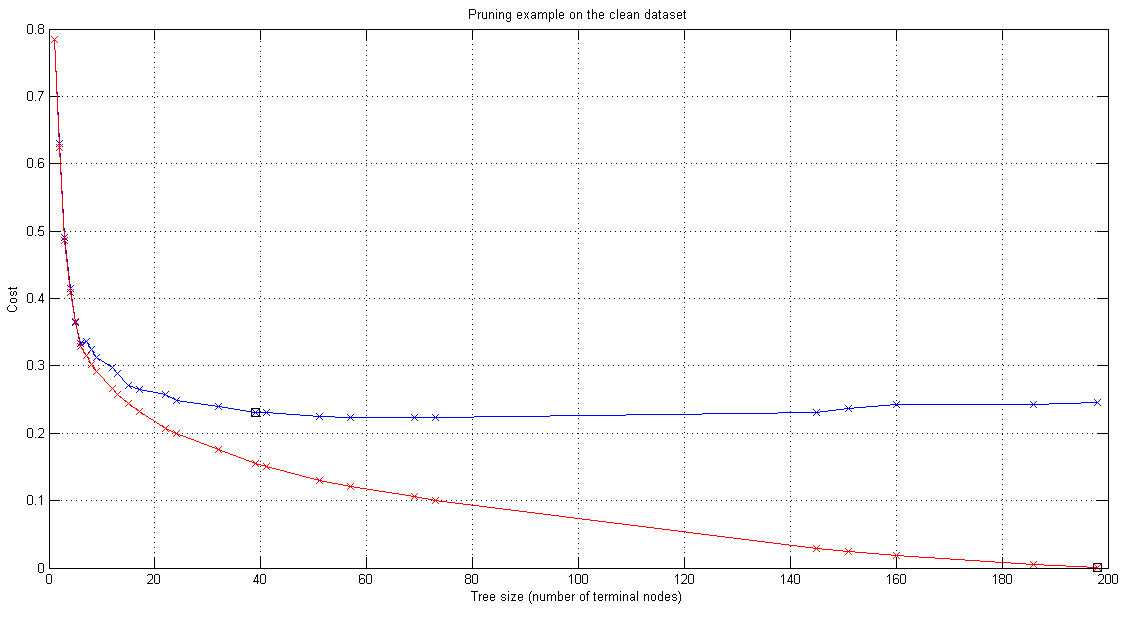
\includegraphics[width=1\columnwidth]{pruneClean} % Example image
\caption{Pruning example on the \emph{clean} dataset}
\label{pruneClean}
\end{figure}

\begin{figure}[H]
\center
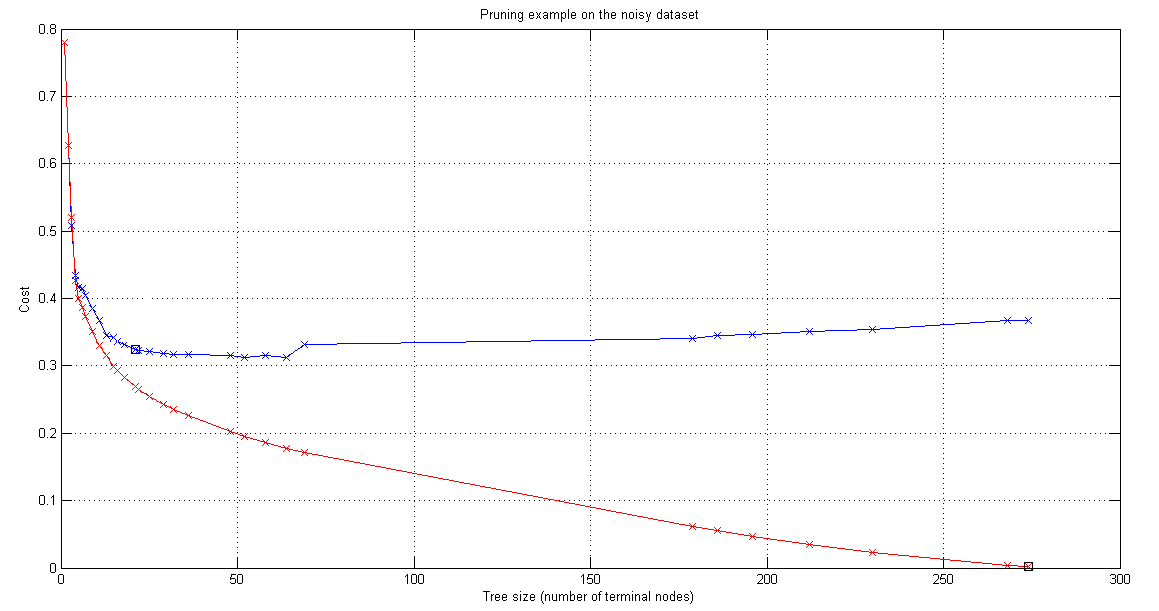
\includegraphics[width=1\columnwidth]{pruneNoisy} % Example image
\caption{Pruning example on the \emph{noisy} dataset}
\label{pruneNoisy}
\end{figure}

\clearpage

%----------------------------------------------------------------------------------------
%	SECTION 5 - Code Flowchart
%----------------------------------------------------------------------------------------

\section{Code Flowchart}

\clearpage

%----------------------------------------------------------------------------------------

\end{document}